\chapter{Principle of Virtual Displacements}
\label{ch:pvd1}

\section{Virtual work principles}
The virtual work principles include the principle of virtual displacements (PVD) and the principle of virtual forces (PVF). It is often that the principle of virtual displacements is referred to as the principle of virtual work and the principle of virtual forces is referred to as the principle of complementary virtual work. In this chapter, we will discuss the principle of virtual displacements or the principle of virtual work, which represents equivalently the \emph{equilibrium equations} of a system. In Ch.~\ref{ch:pvf}, we shall then discuss the principle of virtual forces or the principle of complementary virtual work, which represents equivalently the \emph{compatibility equations} of a system.

\section{The principle of virtual displacements (PVD)}
\topic{Particles}
\begin{equation}
  \dW = 0 \quad\Longleftrightarrow\quad \text{Equilibrium equations: } \sum F_x = \sum F_y = \sum F_z = 0
\end{equation}
where $\dW$ is the external virtual work defined as
\begin{equation}
  \dW = \Bigl(\sum\F\Bigr)\bullet\delta\mat{u} = \Bigl(\sum F_x\Bigr)\delta u_x + \Bigl(\sum F_y\Bigr)\delta u_y + \Bigl(\sum F_z\Bigr)\delta u_z
\end{equation}
with $\delta u_x$, $\delta u_y$, and $\delta u_z$ being the virtual displacements along the $x$-, $y$-, and $z$-axis.

\topic{Rigid bodies}
\begin{equation}
  \begin{aligned}
    \dW = 0 \quad\Longleftrightarrow\quad &\text{Equilibrium equations: }\\
    &\sum F_x = \sum F_y = \sum F_z = 0\ \text{ and }\ \sum M_x = \sum M_y = \sum M_z = 0
  \end{aligned}
\end{equation}
where
\begin{equation}
  \begin{aligned}
    \dW = \Bigl(\sum\F\Bigr)\bullet\delta\mat{u} + \Bigl(\sum\mat{M}\Bigr)\bullet\delta\bs{\theta}
    &= \Bigl(\sum F_x\Bigr)\delta u_x + \Bigl(\sum F_y\Bigr)\delta u_y + \Bigl(\sum F_z\Bigr)\delta u_z\\
    &\quad + \Bigl(\sum M_x\Bigr)\delta\theta_x + \Bigl(\sum M_y\Bigr)\delta\theta_y + \Bigl(\sum M_z\Bigr)\delta\theta_z
  \end{aligned}
\end{equation}
For both particles and rigid bodies, if the equilibrium equations are satisfied, then $\dW = 0$ is readily seen. Conversely, if $\dW = 0$, it is easy to conclude that the equilibrium equations are satisfied because the virtual displacements $\delta u_x$, $\delta u_y$, and $\delta u_z$, and virtual rotations $\delta\theta_x$, $\delta\theta_y$, and $\delta\theta_z$ are independent and arbitrary. Therefore, the principle is proved.

\topic{Deformable bodies}
\begin{keypoint}
With \emph{kinematically admissible} virtual displacement fields $\delta\mat{u}(\mat{x})$,
\begin{equation*}
  \dW = \dU_i \quad\Longleftrightarrow\quad \text{Equilibrium equations}
\end{equation*}
\end{keypoint}
Virtual displacement fields are called kinematically admissible if the following two conditions are satisfied:
\begin{enumerate}[label=(\arabic*)]
  \item $\delta u_i(\mat{x}) = 0$ for $\mat{x}\in S_u$, where $S_u =$ the surfaces where displacements are specified.
  \item $\delta\eps_{ij} = \frac12(\delta u_{i,j}+\delta u_{j,i})$ for $\mat{x}\in V$.
\end{enumerate}
Note that for structural systems, virtual displacements should satisfy the \emph{homogeneous form} of the essential (or geometric) boundary conditions.

The external virtual work $\dW$ is defined as
\begin{equation}
  \dW = \int_{S_t}\bar{\mat{t}}\bullet\delta\mat{u}\,dS + \int_V\bar{\mat{f}}\bullet\delta\mat{u}\,dV
      = \int_{S_t}\bar t_i\,\delta u_i\,dS + \int_V\bar f_i\,\delta u_i\,dV
\end{equation}
where $S_t =$ the surfaces where tractions are specified, and $\bar{\mat{t}}$ and $\bar{\mat{f}} =$ the specified tractions and body forces, respectively.

The virtual internal energy $\dU_i$ is defined as
\begin{equation}
  \dU_i = \int_V\sigma_{ij}\,\delta\eps_{ij}\,dV
\end{equation}
\begin{fig}
  % Boundary element of a deformable body: stresses and surface tractions
\begin{tikzpicture}[scale=1.0,font=\small]
  % body
  \draw[thick] plot[smooth cycle,tension=0.8] coordinates {(0,0) (1.6,-0.6) (3.2,0.2) (3.0,1.6) (1.4,2.2) (-0.2,1.4)};
  \fill[hatch] (2.55,1.55) -- (3.05,1.35) -- (2.85,1.05) -- cycle;
  \foreach \x in {1.9,2.2,...,3.1}{\draw (\x,-0.35) -- (\x-0.2,-0.6);}
  \draw[->] (3.1,1.5) .. controls (4.2,2.2) and (5.4,2.0) .. (6.0,1.4);
  % wedge element
  \begin{scope}[shift={(6.6,-0.2)}]
    \draw[thick] (0,0) -- (0,1.8) -- (1.4,0) -- cycle;
    \draw[load] (0,0.9) -- (-1.2,0.9) node[left] {$\sigma_{xx}$};
    \draw[load] (0,0.75) -- (0,-0.5) node[below left] {$\sigma_{xy}$};
    \draw[load] (0.7,0) -- (0.7,-1.2) node[below] {$\sigma_{yy}$};
    \draw[load] (0.55,0) -- (-0.5,0) node[below left] {$\sigma_{xy}$};
    \draw[->,thick] (0.7,0.9) -- (1.7,1.7) node[above right] {$\mat{n}$};
    \draw[load] (0.7,0.9) -- (0.7,2.2) node[above] {$\bar t_y$};
    \draw[load] (0.7,0.9) -- (2.0,0.9) node[right] {$\bar t_x$};
  \end{scope}
\end{tikzpicture}

\end{fig}
\begin{align*}
  \textstyle\sum F_x = 0:&\qquad \sigma_{xx}\cdot n_x + \sigma_{xy}\cdot n_y = \bar t_x\\
  \textstyle\sum F_y = 0:&\qquad \sigma_{xy}\cdot n_x + \sigma_{yy}\cdot n_y = \bar t_y
\end{align*}

\begin{proof}
\textbf{Part I: Equilibrium equations $\Rightarrow$ $\dW = \dU_i$.}\\
Equilibrium equations:
\begin{equation*}
  \sigma_{ij,j} + \bar f_i = 0\ \text{ in } V \qquad\text{and}\qquad \sigma_{ij}n_j = \bar t_i\ \text{ on } S_t
\end{equation*}
\begin{equation*}
  \begin{aligned}
    \dU_i &= \int_V\sigma_{ij}\delta\eps_{ij}\,dV = \int_V\sigma_{ij}\tfrac12(\delta u_{i,j}+\delta u_{j,i})\,dV = \int_V\sigma_{ij}\delta u_{i,j}\,dV\quad(\because\sigma_{ij}\text{ is symmetric})\\
          &= \int_V(\sigma_{ij}\delta u_i)_{,j}\,dV - \int_V\sigma_{ij,j}\delta u_i\,dV\\
          &= \int_S\sigma_{ij}n_j\,\delta u_i\,dS - \int_V\sigma_{ij,j}\delta u_i\,dV = \int_{S_t}\sigma_{ij}n_j\,\delta u_i\,dS - \int_V\sigma_{ij,j}\delta u_i\,dV\quad(\because\delta u_i = 0\text{ on }S_u)
  \end{aligned}
\end{equation*}
Making use of the two equilibrium equations yields:
\begin{equation*}
  \dU_i = \int_{S_t}\bar t_i\,\delta u_i\,dS + \int_V\bar f_i\,\delta u_i\,dV
\end{equation*}
Therefore $\dU_i = \dW$.

\textbf{Part II: $\dW = \dU_i$ $\Rightarrow$ Equilibrium equations.}\\
From the expression for $\dU_i$ given in Part I, $\dW = \dU_i$ can be written as
\begin{equation*}
  \int_{S_t}\bar t_i\delta u_i\,dS + \int_V\bar f_i\delta u_i\,dV = \int_{S_t}\sigma_{ij}n_j\delta u_i\,dS + \int_V(-\sigma_{ij,j})\delta u_i\,dV
\end{equation*}
or
\begin{equation*}
  \int_{S_t}(\bar t_i - \sigma_{ij}n_j)\delta u_i\,dS + \int_V(\bar f_i + \sigma_{ij,j})\delta u_i\,dV = 0
\end{equation*}
Because the virtual displacements are arbitrary, the above identity results in (choose $\delta u_i$ as a delta function on $S_t$ or in $V$):
\begin{equation*}
  \sigma_{ij}n_j = \bar t_i\ \text{ on } S_t,\qquad \sigma_{ij,j}+\bar f_i = 0\ \text{ in } V
\end{equation*}
which are the equilibrium equations (one is on the boundary and the other is in the body).
\end{proof}

We shall notice that the principle of virtual displacements has nothing to do with constitutive laws and therefore can be applied to all kinds of materials, elastic, inelastic, etc. For an inelastic body,
\begin{equation}
  \dU_i = \int_V\sigma_{ij}\delta\eps_{ij}\,dV = \int_V\sigma_{ij}(\delta\eps^e_{ij}+\delta\eps^i_{ij})\,dV = \dU + \dU_d
\end{equation}
where $\delta\eps^e_{ij} =$ virtual elastic strains and $\delta\eps^i_{ij} =$ virtual inelastic strains, $\dU =$ virtual strain energy, and $\dU_d =$ virtual dissipation. For example, we often employ the PVD to calculate the limit (collapse) load of structures in conjunction with the upper bound theorem. In this case, we often assume that the rigid plastic law is followed. This means that we neglect $\dU$ and therefore $\dU_i = \dU_d$ and the PVD becomes:
\begin{equation}
  \dW = \dU_d
\end{equation}
\begin{center}
  \begin{minipage}{0.35\linewidth}\centering% Moment-rotation of a rigid-plastic hinge: dissipation (shaded) >> strain energy
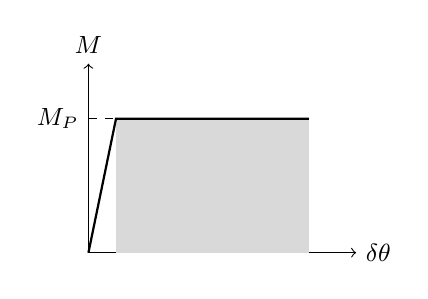
\begin{tikzpicture}[scale=1.0,font=\small]
  \draw[->] (0,0) -- (3.4,0) node[right] {$\delta\theta$};
  \draw[->] (0,0) -- (0,2.4) node[above] {$M$};
  \fill[black!15] (0.35,0) -- (0.35,1.7) -- (2.8,1.7) -- (2.8,0) -- cycle;
  \draw[thick] (0,0) -- (0.35,1.7) -- (2.8,1.7);
  \draw[dashed] (0,1.7) -- (0.35,1.7); \node[left] at (0,1.7) {$M_P$};
\end{tikzpicture}
\end{minipage}\hfill
  \begin{minipage}{0.6\linewidth}The energy dissipation due to plastic work (shaded area) is much larger than the strain energy.\end{minipage}
\end{center}

\section{The principle of stationary (minimum) total potential energy and Castigliano's first theorem}
\topic{Elastic bodies}
There exists a strain energy function $U$ such that $\dU = \dU_i$ for elastic bodies. The strain energy is a function of displacements or positions only and is independent of how the body is deformed to this position. Notice that the existence of $U$ does not require the body to be linear. For the special case of linearly elastic materials, $U$ is a quadratic function of displacements or strains.

\topic{Strain energy for structural members}
\begin{align*}
  \text{Axial deformation:}& \quad U = \tfrac12\int EA\,u'^2\,dx\\
  \text{Flexural deformation:}& \quad U = \tfrac12\int EI\,v''^2\,dx\\
  \text{Torsional deformation:}& \quad U = \tfrac12\int GJ\,\theta_x'^2\,dx
\end{align*}

\topic{Conservative forces}
A conservative force is defined as a force that the work done by the force is independent of the path along which it travels. Therefore, the work done is only dependent on the initial and final positions. In this case, there exists a load potential $V$, a function of positions only, such that $\dW = -\delta V$.

\topic{Conservative systems and total potential energy}
If a body is elastic (conservative internally) and the external forces are conservative (conservative externally), the system (internal plus external) is called conservative. For a conservative system, the PVD then becomes
\begin{equation}
  \dU + \delta V = 0
\end{equation}
Define the total potential energy as $\Pi = U + V$; the PVD becomes
\begin{equation}
  \delta\Pi = 0
\end{equation}
This is often called the \emph{principle of stationary total potential energy} or the \emph{principle of minimum total potential energy}.

\topic{Examples of total potential energy}
Total potential energy $\Pi = U + V$.
\begin{fig}
  % Linear spring subjected to P
\begin{tikzpicture}[scale=1.0,font=\small]
  \fill[left color=black!60,right color=black!15] (-0.3,-0.4) rectangle (0,0.4);
  \draw[thick,decorate,decoration={zigzag,segment length=6pt,amplitude=4pt,pre length=4pt,post length=4pt}] (0,0) -- (3,0);
  \node[above] at (1.5,0.3) {$K$};
  \draw[load] (3.2,0) -- (4.2,0) node[right] {$P(\Delta)$};
\end{tikzpicture}

\end{fig}
\begin{gather*}
  \Pi = U + V = \tfrac12 K\Delta^2 - P\Delta\\
  \delta\Pi = K\Delta\cdot\delta\Delta - P\cdot\delta\Delta = (K\Delta - P)\delta\Delta = 0\\
  \Rightarrow K\Delta = P
\end{gather*}
\begin{fig}
  % Beam with distributed load, point load, end moment, inclined bar and spring
\begin{tikzpicture}[scale=0.85,font=\small]
  \def\L{3.2}
  \pic at (0,0) {wallL};
  \draw[member] (0,0) -- (3*\L,0);
  \node[above] at (1.6*\L,0.1) {$EI$};
  % distributed load on first span
  \foreach \x in {0.2,0.55,...,3.0}{\draw[->] (\x,0.9) -- (\x,0.12);} \draw (0.2,0.9) -- (3.0,0.9);
  \node[above] at (1.6,0.95) {$w$};
  \draw[->] (0,1.2) -- (0,2.4) node[right] {$v(x)$};
  % point load at 2L
  \draw[load] (2*\L,1.8) -- (2*\L,0.15) node[pos=0,above] {$\overline{P}$};
  % end moment at 3L
  \draw[->,thick] (3*\L+0.5,0.55) arc (40:200:0.5); \node[above left] at (3*\L-0.3,0.7) {$\overline{M}$};
  % inclined bar at 30 deg from vertical, up-right from the end
  \coordinate (E) at (3*\L,0);
  \coordinate (T) at ($(E)+(60:2.8)$);
  \draw[thinmember] (E) -- (T);
  \pic[rotate=60] at (T) {wallR};
  \node[left] at ($(E)!0.5!(T)+(-0.1,0.1)$) {$EA$};
  \draw[dashed] (E) -- ($(E)+(0,2.2)$);
  \draw[->] ($(E)+(0,1.4)$) arc (90:60:1.4); \node at ($(E)+(0.45,1.75)$) {$30^\circ$};
  \draw[dim] ($(E)+(0.9,0.2)$) -- ($(T)+(0.9,0.2)$) node[midway,right] {$L$};
  % spring below the end
  \draw[thick,decorate,decoration={zigzag,segment length=6pt,amplitude=4pt,pre length=6pt,post length=6pt}] (E) -- ($(E)+(0,-2.6)$);
  \node[right] at ($(E)+(0.2,-1.6)$) {$K_0$};
  \pic at ($(E)+(0,-2.6)$) {fixed};
  % dims
  \draw[dim] (0,-0.9) -- (\L,-0.9) node[midway,fill=white,inner sep=1pt] {$L$};
  \draw[dim] (\L,-0.9) -- (2*\L,-0.9) node[midway,fill=white,inner sep=1pt] {$L$};
  \draw[dim] (2*\L,-0.9) -- (3*\L,-0.9) node[midway,fill=white,inner sep=1pt] {$L$};
  \foreach \x in {0,\L,2*\L,3*\L}{\draw (\x,-0.7) -- (\x,-1.1);}
\end{tikzpicture}

\end{fig}
\begin{gather*}
  U = \frac12\int_0^{3L}EIv''^2\,dx + \frac12\frac{EA}{L}\Delta^2 + \frac12K_0\bigl[v(3L)\bigr]^2\\
  \Delta = -\frac{\sqrt3}{2}v(3L)\quad(\text{``$-$'' means shortening})\\
  V = \int_0^L -w\cdot v(x)\,dx + \overline{P}\cdot v(2L) - \overline{M}\cdot v'(3L)
\end{gather*}

\topic{Rayleigh--Ritz method}
Let the displacement field be constructed through the use of some functions, $\phi_i(x)$ ($i = 1, n$), e.g., $v(x) = \sum_{i=1}^n c_i\phi_i(x)$, where $c_i =$ generalized coefficients. Substituting $v(x)$ into $\Pi$ results in $\Pi(\mat{c}) = U(\mat{c}) + V(\mat{c})$. Then according to the principle of stationary total potential energy,
\begin{equation}
  \delta\Pi = \sum_{i=1}^n\pd{\Pi}{c_i}\delta c_i = 0 \quad\Rightarrow\quad \pd{\Pi}{c_i} = 0,\ i = 1, n \quad\because\delta c_i\text{ are independent}
\end{equation}
The load potential can be expressed as a linear function of $\mat{c}$, $V(\mat{c}) = -\mat{c}^\tr\Pvec_c$, where $\Pvec_c$ is called the generalized load vector. When the material is linearly elastic, the strain energy is a quadratic function of $\mat{c}$, $U(\mat{c}) = \frac12\mat{c}^\tr\Kmat_c\mat{c}$, where $\Kmat_c$ is called the generalized stiffness matrix. With these definitions, the expression $\pd{\Pi}{\mat{c}} = \mat{0}$ becomes
\begin{equation}
  \Kmat_c\mat{c} = \Pvec_c
\end{equation}

\topic{Castigliano's first theorem}
When the external forces $\Pvec$ acting on a structural system are point loads or concentrated loads (including couples), then the strain energy and the load potential can be expressed as functions of the corresponding displacements (including rotations) $\bs{\Delta}$ as
\begin{equation}
  U = U(\Delta_1, \Delta_2, \dots, \Delta_n)\quad\text{and}\quad V = -\sum_{i=1}^n P_i\Delta_i
\end{equation}
According to the principle of stationary total potential energy, we obtain
\begin{equation}
  \delta\Pi = \sum_{i=1}^n\pd{U}{\Delta_i}\delta\Delta_i - \sum_{i=1}^n P_i\delta\Delta_i = \sum_{i=1}^n\Bigl(\pd{U}{\Delta_i} - P_i\Bigr)\delta\Delta_i = 0
\end{equation}
As $\delta\bs{\Delta}$ are independent and arbitrary, we conclude from the above equation that
\begin{equation}
  \pd{U}{\Delta_i} = P_i,\quad i = 1, n
\end{equation}
This is often referred to as \emph{Castigliano's first theorem}. Note that the theorem can be applied to nonlinearly elastic material as well. In this case, $U$ is not a quadratic function of $\bs{\Delta}$.

The stiffness equations for a linear structural system can be derived from the principle of stationary total potential energy or Castigliano's first theorem. The strain energy and load potential are of the form:
\begin{equation}
  U = \tfrac12\bs{\Delta}^\tr\Kmat\bs{\Delta}\quad\text{and}\quad V = -\bs{\Delta}^\tr\Pvec
\end{equation}
Therefore, from $\delta\Pi = 0$ (or $\partial\Pi/\partial\Delta_i = 0$ or $\partial\Pi/\partial\bs{\Delta} = \mat{0}$) or $\partial U/\partial\Delta_i = P_i$ ($\partial U/\partial\bs{\Delta} = \Pvec$), we have
\begin{equation}
  \Kmat\bs{\Delta} = \Pvec
\end{equation}

\topic{Example of Castigliano's first theorem (nonlinear elastic case)}
\begin{fig}
  % Nonlinear elastic bar subjected to F
\begin{tikzpicture}[scale=1.0,font=\small]
  \fill[left color=black!60,right color=black!15] (-0.3,-0.4) rectangle (0,0.4);
  \draw[thick] (0,-0.15) rectangle (4,0.15);
  \draw[load] (4.1,0) -- (5.0,0) node[right] {$F(\delta)$};
\end{tikzpicture}

\end{fig}
\begin{gather*}
  F = c\cdot\delta^{\frac12}\\
  U = \int_0^\delta F\,d\delta = \int_0^\delta c\cdot\delta^{\frac12}\,d\delta = \frac23 c\cdot\delta^{\frac32}\\
  \pd{U}{\delta} = c\cdot\delta^{\frac12} = F
\end{gather*}

\begin{example}[Plastic collapse load or limit load of beams]
Determine this structure's plastic collapse load by P.V.W.
\begin{fig}
  % Propped cantilever with two point loads W at the third points
\begin{tikzpicture}[scale=1.0,font=\small]
  \def\L{9}
  \pic at (0,0) {wallL}; \pic at (\L,0) {pin};
  \draw[member] (0,0) -- (\L,0);
  \node[below right] at (0,0) {$A$}; \node[below] at (3,-0.05) {$B$}; \node[below] at (6,-0.05) {$C$}; \node[below left] at (\L,0) {$D$};
  \draw[load] (3,1.6) -- (3,0.15) node[pos=0,above] {$W$};
  \draw[load] (6,1.6) -- (6,0.15) node[pos=0,above] {$W$};
  \draw[dim] (0,-0.9) -- (3,-0.9) node[midway,fill=white,inner sep=1pt] {$\frac L3$};
  \draw[dim] (3,-0.9) -- (6,-0.9) node[midway,fill=white,inner sep=1pt] {$\frac L3$};
  \draw[dim] (6,-0.9) -- (\L,-0.9) node[midway,fill=white,inner sep=1pt] {$\frac L3$};
  \foreach \x in {0,3,6,\L}{\draw (\x,-0.7) -- (\x,-1.1);}
\end{tikzpicture}

\end{fig}
\underline{Mechanism 1:} nodes $A$ and $C$ become plastic hinges.
\begin{fig}
  % Mechanism 1: plastic hinges at A and C
\begin{tikzpicture}[scale=1.0,font=\small]
  \pic at (0,0) {wallL}; \pic at (9,0) {pin};
  \draw[thick] (0,0) -- (9,0);
  \draw[dashed,thick] (0,0) -- (6,-1.2) -- (9,0);
  \node[node dot] at (0,0) {}; \node[node dot] at (6,-1.2) {};
  \draw[->] (2.2,0) arc (0:-11.3:2.2); \node[right] at (2.3,-0.3) {$\delta\theta$};
\end{tikzpicture}

\end{fig}
\begin{equation*}
  \dW = W\Bigl(\frac L3\delta\theta\Bigr) + W\Bigl(\frac{2L}{3}\delta\theta\Bigr) = WL\delta\theta
\end{equation*}
and virtual dissipation
\begin{equation*}
  \dU_d = M_p\delta\theta + M_p(3\delta\theta) = 4M_p\delta\theta
\end{equation*}
where $M_p =$ sectional plastic moment or moment capacity. By P.V.W., we have
\begin{equation*}
  WL\delta\theta = 4M_p\delta\theta \Rightarrow W = \frac{4M_p}{L}
\end{equation*}
\underline{Mechanism 2:} nodes $A$ and $B$ become plastic hinges.
\begin{fig}
  % Mechanism 2: plastic hinges at A and B
\begin{tikzpicture}[scale=1.0,font=\small]
  \pic at (0,0) {wallL}; \pic at (9,0) {pin};
  \draw[thick] (0,0) -- (9,0);
  \draw[dashed,thick] (0,0) -- (3,-1.2) -- (9,0);
  \node[node dot] at (0,0) {}; \node[node dot] at (3,-1.2) {};
  \draw[->] (6.8,0) arc (180:191.3:2.2); \node[left] at (6.7,-0.3) {$\delta\theta$};
\end{tikzpicture}

\end{fig}
\begin{equation*}
  \dW = W\Bigl(\frac L3 2\delta\theta\Bigr) + W\Bigl(\frac L3\delta\theta\Bigr) = WL\delta\theta
\end{equation*}
and virtual dissipation
\begin{equation*}
  \dU_d = M_p(2\delta\theta) + M_p(3\delta\theta) = 5M_p\delta\theta
\end{equation*}
By P.V.W., we have
\begin{equation*}
  WL\delta\theta = 5M_p\delta\theta \Rightarrow W = \frac{5M_p}{L}
\end{equation*}
\underline{Mechanism 3:} nodes $B$ and $C$ become plastic hinges.
\begin{fig}
  % Mechanism 3: plastic hinges at B and C
\begin{tikzpicture}[scale=1.0,font=\small]
  \pic at (0,0) {wallL}; \pic at (9,0) {pin};
  \draw[thick] (0,0) -- (9,0);
  \draw[dashed,thick] (3,0) -- (6,-1.2) -- (9,0);
  \node[node dot] at (3,0) {}; \node[node dot] at (6,-1.2) {};
  \draw[->] (4.6,0) arc (0:-21.8:1.6); \node[right] at (4.7,-0.35) {$\delta\theta$};
\end{tikzpicture}

\end{fig}
\begin{equation*}
  \dW = W\Bigl(\frac L3\delta\theta\Bigr) = \frac{WL}{3}\delta\theta
\end{equation*}
and virtual dissipation
\begin{equation*}
  \dU_d = M_p\delta\theta + M_p(2\delta\theta) = 3M_p\delta\theta
\end{equation*}
By P.V.W., we have
\begin{equation*}
  \frac{WL}{3}\delta\theta = 3M_p\delta\theta \Rightarrow W = \frac{9M_p}{L}
\end{equation*}
According to the upper bound theory, the collapse load shall be the minimum of these three values. However, it doesn't mean that the real collapse load is the minimum one according to the upper bound theorem. We can plot the moment diagram for the mechanism with the minimum failure load. If there is no section that violates the yield condition, then the upper bound solution is also the exact one; try to draw the moment diagrams for the above three mechanisms. You will find that the internal moments for mechanism 1 are all less than or equal to $M_p$. Therefore, $W = \dfrac{4M_p}{L}$ is the exact failure load. However, some of the internal moments for mechanisms 2 and 3 are greater than $M_p$.
\end{example}

\begin{example}[Braced frame]
Find the plastic collapse load in terms of $M_p$ and $L$. Note that $ac$ is an axial bar with the axial capacity of $A\sigma_y$, which is equal to $\dfrac{M_p}{L}$.
\begin{fig}
  % Braced frame: geometry (left) and collapse mechanism (right)
\begin{tikzpicture}[scale=0.8,font=\small]
  % ---- geometry ----
  \begin{scope}
    \coordinate (a) at (0,0); \coordinate (b) at (0,3); \coordinate (c) at (4,3); \coordinate (d) at (4,-2);
    \draw[member] (a) -- (b) -- (c) -- (d); \draw[thinmember] (a) -- (c);
    \pic at (a) {pin}; \pic at (d) {pin};
    \node[left] at (a) {a}; \node[above left] at (b) {b}; \node[above right] at (c) {c}; \node[right] at (d) {d};
    \draw[load] (c) -- ++(1.4,0) node[right] {P};
    \node[above] at (2,3.05) {$2M_p$}; \node[below] at (2,2.95) {$4L$};
    \node[left,align=right] at (-0.1,1.5) {$3M_p$\\$3L$};
    \node[right,align=left] at (4.1,0.5) {$M_p$\\$5L$};
    \node[below right] at (1.6,1.2) {$\sigma_y A = \dfrac{M_p}{L}$};
  \end{scope}
  % ---- mechanism ----
  \begin{scope}[xshift=9cm]
    \coordinate (a) at (0,0); \coordinate (b) at (-0.6,3); \coordinate (c) at (3.4,3.2); \coordinate (d) at (4,-2);
    \draw[thinmember] (a) -- (b) -- (c) -- (d);
    \pic at (a) {pin}; \pic at (d) {pin};
    \draw[dashed] (a) -- (0,3.2); \draw[dashed] (d) -- (4,3.4);
    \draw[->] (0,1.2) arc (90:101.3:1.2); \node[left] at (-0.3,1.5) {$\delta\theta$};
    \draw[->] (4,1.0) arc (90:96.8:3.0); \node[left] at (3.85,0.9) {$\frac35\delta\theta$};
    \draw[load] (c) -- ++(1.4,0) node[right] {P};
    \draw[->] (b) -- ++(1.0,0) node[above] {$3L\delta\theta$}; \draw[->] (c) -- ++(1.0,0.2) ; \node[above] at (3.8,3.5) {$3L\delta\theta$};
    \draw[load] ($(a)!0.55!(c)$) -- ++(-0.6,-0.5); \node[right] at ($(a)!0.55!(c)+(0.1,0.2)$) {$\frac{M_p}{L}$};
    \draw[load] ($(a)!0.1!(c)$) -- ++(0.6,0.5);
  \end{scope}
\end{tikzpicture}

\end{fig}
\begin{align*}
  \dU_d &= 2M_p(\delta\theta) + M_p\Bigl(\frac35\delta\theta\Bigr) &&\text{or}& \dU_d &= 2M_p(\delta\theta) + M_p\Bigl(\frac35\delta\theta\Bigr) + \frac{M_p}{L}\Bigl(\frac45 3L\delta\theta\Bigr)\\
  \dW &= P(3L\delta\theta) - \frac{M_p}{L}\Bigl(\frac45 3L\delta\theta\Bigr) &&\text{or}& \dW &= P(3L\delta\theta)
\end{align*}
Note the former case considers the axial bar effect as applied loads while the latter treats it as internal forces.
\begin{equation*}
  \dU_d = \dW \;\rightarrow\; P = \frac{5M_p}{3L}.\qquad\text{Without the brace, } P = \frac{2.6M_p}{3L} < \frac{5M_p}{3L},\text{ which is expected.}
\end{equation*}
\end{example}

\begin{example}[Portal frame]
\leavevmode
\begin{fig}
  % Portal frame: (a) loading and (b)-(d) collapse mechanisms
\begin{tikzpicture}[scale=0.75,font=\footnotesize]
  % ---- (a) ----
  \begin{scope}
    \draw[member] (0,0) -- (0,3) -- (5,3) -- (5,0);
    \pic at (0,0) {fixed}; \pic at (5,0) {fixed};
    \node[below] at (0,-0.3) {$A$}; \node[below] at (5,-0.3) {$D$};
    \node[above left] at (0,3) {$B$}; \node[above right] at (5,3) {$C$}; \node[below] at (2.5,2.9) {$E$};
    \draw[load] (-1.2,3) -- (-0.1,3) node[pos=0,above] {$P$};
    \draw[load] (2.5,4.3) -- (2.5,3.1) node[pos=0,right] {$2P$};
    \node[above] at (1.4,3.05) {$2M_p$}; \node[right] at (0.05,1.5) {$M_p$}; \node[left] at (4.95,1.5) {$M_p$};
    \draw[dim] (0,4.6) -- (2.5,4.6) node[midway,fill=white,inner sep=1pt] {$l/2$};
    \draw[dim] (2.5,4.6) -- (5,4.6) node[midway,fill=white,inner sep=1pt] {$l/2$};
    \draw[dim] (-1.6,0) -- (-1.6,3) node[midway,left] {$0.6l$};
    \node at (2.5,-1.1) {(a)};
  \end{scope}
  % ---- (b) beam mechanism ----
  \begin{scope}[xshift=8.5cm]
    \draw[member] (0,0) -- (0,3) -- (2.5,2.2) -- (5,3) -- (5,0);
    \pic at (0,0) {fixed}; \pic at (5,0) {fixed};
    \node[node dot] at (0,3) {}; \node[node dot] at (2.5,2.2) {}; \node[node dot] at (5,3) {};
    \node[below] at (0,-0.3) {$A$}; \node[below] at (5,-0.3) {$D$};
    \node[above left] at (0,3) {$B$}; \node[above right] at (5,3) {$C$}; \node[below] at (2.5,2.1) {$E$};
    \draw[load] (-1.2,3) -- (-0.1,3) node[pos=0,above] {$P_{c1}$};
    \draw[load] (2.5,3.5) -- (2.5,2.3) node[pos=0,right] {$2P_{c1}$};
    \draw[->] (1.2,3) arc (0:-17.7:1.2); \node[above] at (1.0,2.95) {$\theta$};
    \draw[->] (3.8,3) arc (180:197.7:1.2); \node[above] at (4.0,2.95) {$\theta$};
    \node[below] at (2.5,1.5) {$2\theta$};
    \draw[dim] (5.6,2.2) -- (5.6,3) node[midway,right] {$\frac{l\theta}{2}$};
    \node at (2.5,-1.1) {(b)};
  \end{scope}
  % ---- (c) sway mechanism ----
  \begin{scope}[yshift=-7.5cm]
    \draw[member] (0,0) -- (0.6,3) -- (5.6,3) -- (5,0);
    \pic at (0,0) {fixed}; \pic at (5,0) {fixed};
    \node[node dot] at (0,0) {}; \node[node dot] at (0.6,3) {}; \node[node dot] at (5.6,3) {}; \node[node dot] at (5,0) {};
    \node[below] at (0,-0.3) {$A$}; \node[below] at (5,-0.3) {$D$};
    \node[above left] at (0.6,3) {$B$}; \node[above right] at (5.6,3) {$C$}; \node[below] at (3.1,2.9) {$E$};
    \draw[load] (-0.7,3) -- (0.5,3) node[pos=0,above] {$P_{c2}$};
    \draw[load] (3.1,4.3) -- (3.1,3.1) node[pos=0,right] {$2P_c$};
    \draw[dashed] (0,0) -- (0,3.3); \draw[dashed] (5,0) -- (5,3.3);
    \draw[dim] (0,3.8) -- (0.6,3.8) node[midway,above] {$0.6l\theta$};
    \node[right] at (0.4,1.6) {$\theta$}; \node[left] at (4.6,1.6) {$\theta$};
    \node at (2.5,-1.1) {(c)};
  \end{scope}
  % ---- (d) combined mechanism ----
  \begin{scope}[xshift=8.5cm,yshift=-7.5cm]
    \draw[member] (0,0) -- (0.6,3) -- (3.1,2.2) -- (5.6,3) -- (5,0);
    \pic at (0,0) {fixed}; \pic at (5,0) {fixed};
    \node[node dot] at (0,0) {}; \node[node dot] at (3.1,2.2) {}; \node[node dot] at (5.6,3) {}; \node[node dot] at (5,0) {};
    \node[below] at (0,-0.3) {$A$}; \node[below] at (5,-0.3) {$D$};
    \node[above left] at (0.6,3) {$B$}; \node[above right] at (5.6,3) {$C$}; \node[below] at (3.1,2.1) {$E$};
    \draw[load] (-0.7,3) -- (0.5,3) node[pos=0,above] {$P_{c3}$};
    \draw[load] (3.1,3.5) -- (3.1,2.3) node[pos=0,right] {$2P_c$};
    \draw[dashed] (0,0) -- (0,3.3); \draw[dashed] (5,0) -- (5,3.3);
    \draw[dim] (0,3.8) -- (0.6,3.8) node[midway,above] {$0.6l\theta$};
    \draw[dim] (-0.8,2.2) -- (-0.8,3) node[midway,left] {$\frac{l\theta}{2}$};
    \node[right] at (0.4,1.6) {$\theta$}; \node[left] at (4.6,1.2) {$\theta$};
    \node[below] at (3.1,1.5) {$2\theta$}; \node[above] at (4.6,2.7) {$2\theta$};
    \node at (2.5,-1.1) {(d)};
  \end{scope}
\end{tikzpicture}

\end{fig}
\begin{enumerate}[label=\alph*.,start=2,leftmargin=*]
  \item $\dW = 2P\bigl(\frac l2\delta\theta\bigr) = Pl\delta\theta$,\quad $\dU_d = M_P(\delta\theta)\times2 + 2M_P(2\delta\theta) = 6M_P\delta\theta$
    \begin{equation*}
      Pl\delta\theta = 6M_P\delta\theta \Rightarrow P = \frac{6M_P}{l}
    \end{equation*}
  \item $\dW = P\bigl(\frac{3l}{5}\delta\theta\bigr)$,\quad $\dU_d = M_P(\delta\theta)\times4 = 4M_P\delta\theta$
    \begin{equation*}
      \frac{3Pl}{5}\delta\theta = 4M_P\delta\theta \Rightarrow P = \frac{20M_P}{3l}
    \end{equation*}
  \item $\dW = P\bigl(\frac{3l}{5}\delta\theta\bigr) + 2P\bigl(\frac l2\delta\theta\bigr) = \frac{8Pl}{5}\delta\theta$,\quad $\dU_d = M_P(\delta\theta)\times2 + M_P(2\delta\theta) + 2M_P(2\delta\theta) = 8M_P\delta\theta$
    \begin{equation*}
      \frac{8Pl}{5}\delta\theta = 8M_P\delta\theta \Rightarrow P = \frac{5M_P}{l}
    \end{equation*}
\end{enumerate}
\end{example}

\begin{example}[Truss]
This example is adopted from the textbook, p.~141, Example~6.1.
\end{example}

\begin{example}[P.V.D.]
\leavevmode
\begin{fig}
  % Cantilever beam AB with a tip load P
\begin{tikzpicture}[scale=1.0,font=\small]
  \pic at (0,0) {wallL};
  \draw[thick] (0,-0.15) rectangle (5,0.15);
  \node[above right] at (0,0.15) {A}; \node[above left] at (5,0.15) {B};
  \draw[->] (0.1,0) -- (1.4,0) node[right] {$x$};
  \draw[->] (0,0.5) -- (0,2.0) node[above] {$Y$};
  \draw[load] (5,0.2) -- (5,1.5) node[above] {$P$};
\end{tikzpicture}

\end{fig}
The exact displacement field is known as $v(x) = \dfrac{P}{EI}\Bigl(L\dfrac{x^2}{2} - \dfrac{x^3}{6}\Bigr)$, which can be obtained by integrating $EIv'' = M(x) = P(L-x)$ twice. Assume the virtual displacement field is $u(x)$, which can be any function of $x$ but shall be kinematically admissible, i.e.\ $u(0) = 0$ and $u'(0) = 0$.

Since
\begin{equation*}
  \dU = \int_0^L EIv''u''\,dx\qquad\text{and}\qquad \dW = Pu_B = Pu(L)
\end{equation*}
By P.V.D., we have
\begin{equation*}
  Pu(L) = \int_0^L EIv''u''\,dx
\end{equation*}
By making use of the kinematically admissible conditions, $u(0) = 0$ and $u'(0) = 0$, and $EIv'' = P(L-x)$, we have
\begin{equation*}
  Pu(L) = \int_0^L P(L-x)u''\,dx
\end{equation*}
We will choose different $u(x)$ to verify the above identity.
\begin{description}[leftmargin=2em]
  \item[Case 1:] $u(x) = \dfrac{u_B}{L^2}x^2$
    \begin{align*}
      \text{LHS} &= Pu_B\\
      \text{RHS} &= \int_0^L P(L-x)\frac{2u_B}{L^2}\,dx = Pu_B
    \end{align*}
  \item[Case 2:] $u(x) = u_B\Bigl(-\cos\dfrac{\pi x}{2L}+1\Bigr)$\\
    That RHS $=$ LHS can be shown easily.
\end{description}
\emph{As the real displacement field is exact, the P.V.D. relationship would be satisfied regardless of the chosen virtual displacement fields. However, if $v(x)$ is not exact, there will be some differences as discussed below.}

Assume $v(x) = \dfrac{v_B}{L^2}x^2$; we would like to find $v_B$.
\begin{description}[leftmargin=2em]
  \item[Case 1:] $u(x) = \dfrac{u_B}{L^2}x^2$
    \begin{align*}
      \text{LHS} &= Pu_B\\
      \text{RHS} &= \frac{4EI}{L^3}u_Bv_B\\
      \because\text{RHS} = \text{LHS} &\Rightarrow v_B = \frac{PL^3}{4EI}\qquad\Bigl(\text{The exact one is } v_B = \frac{PL^3}{3EI}\Bigr)
    \end{align*}
  \item[Case 2:] $u(x) = \dfrac{u_B}{L^4}x^4$
    \begin{align*}
      \text{LHS} &= Pu_B\\
      \text{RHS} &= \frac{8EI}{L^3}u_Bv_B\\
      \because\text{RHS} = \text{LHS} &\Rightarrow v_B = \frac{PL^3}{8EI}
    \end{align*}
\end{description}
\begin{note}
You may prefer to assume $v(x) = cx^2$, where $c$ is to be determined by the PVD. For case 1, you assume $u(x) = x^2$ and for case 2 $u(x) = x^4$. You will get the same solutions; namely $c = \dfrac{PL}{4EI}$ for case 1 and $c = \dfrac{PL}{8EI}$ for case 2. Please check.

When you assume $v(x) = c\Bigl(L\dfrac{x^2}{2} - \dfrac{x^3}{6}\Bigr)$ you will get the same $c = \dfrac{P}{EI}$ for cases 1 and 2, which is the exact solution. Of course, in reality, it is impossible to know the exact function form. We will employ the Rayleigh--Ritz method to solve it by assuming $v(x) = c_1x^2 + c_2x^3$.
\end{note}

\topic{Conclusion}
\begin{enumerate}
  \item The real and virtual displacement fields are independent, but the virtual displacement field should be kinematically admissible.
  \item When the real displacement field is exact, whatever you choose for the virtual displacement field, exact solutions will be obtained from P.V.D.
  \item When the real displacement field is not exact, the solutions (approximate) obtained using P.V.D. depend on the chosen virtual displacement fields. Also, these approximate displacements will be less than the exact ones.
\end{enumerate}
\end{example}

\begin{example}[Rayleigh--Ritz method and PVD]
Solve the above example using the Rayleigh--Ritz method. Assume $v(x) = c_1x^2 + c_2x^3$, which already satisfies the geometric boundary conditions $v(0) = 0$ and $v'(0) = 0$. Then the total potential energy $\Pi$ can be obtained as follows:
\begin{gather*}
  \Pi = U + V\\
  U = \frac12\int EIv''^2\,dx = \frac12EI(4c_1^2L + 12c_1c_2L^2 + 12c_2^2L^3) = \frac12\mat{c}^\tr\Kmat_c\mat{c}\\
  V = -Pv(L) = -P(c_1L^2 + c_2L^3) = -\mat{c}^\tr\Pvec_c\\
  \Pi = \frac12\mat{c}^\tr\Kmat_c\mat{c} - \mat{c}^\tr\Pvec_c
\end{gather*}
$\pd{\Pi}{c_1} = \pd{\Pi}{c_2} = 0$, we have $\Kmat_c\mat{c} = \Pvec_c$ or
\begin{equation*}
  EI\bmat{4L & 6L^2\\ 6L^2 & 12L^3}\Bmat{c_1\\ c_2} = \Bmat{PL^2\\ PL^3}
  \;\Rightarrow\; \Bmat{c_1\\ c_2} = \frac{P}{EI}\Bmat{L/2\\ -1/6}
  \;\Rightarrow\; v(x) = \frac{P}{EI}\Bigl(\frac L2x^2 - \frac16x^3\Bigr)
\end{equation*}
\begin{note}
In terms of computational efforts, the PVD
\begin{equation*}
  \dW = \dU\qquad \dW = Pu(L)\qquad \dU = \int_0^L EIv''u''\,dx
\end{equation*}
is more effective to use. Let $v(x) = c_1x^2 + c_2x^3$ and

Case 1: $u(x) = x^2$:\quad $PL^2 = \int_0^L EI(2c_1+6c_2x)(2)\,dx \Rightarrow PL^2 = EI(4c_1L + 6c_2L^2)$\\
\phantom{Case 1: }$u(x) = x^3$:\quad $PL^3 = \int_0^L EI(2c_1+6c_2x)(6x)\,dx \Rightarrow PL^3 = EI(6c_1L^2 + 12c_2L^3)$\\
the same system as above.

Case 2: $u(x) = x^4$ and $x^5$
\begin{equation*}
  EI\bmat{8L^3 & 18L^4\\ 10L^4 & 24L^5}\Bmat{c_1\\ c_2} = \Bmat{PL^4\\ PL^5}
  \;\Rightarrow\; \Bmat{c_1\\ c_2} = \frac{P}{EI}\Bmat{L/2\\ -1/6}
  \;\Rightarrow\; v(x) = \frac{P}{EI}\Bigl(\frac L2x^2 - \frac16x^3\Bigr)
\end{equation*}
You shall be aware that if $u(x)$ (virtual displacement) has the same form as $v(x)$ the system matrix is symmetric; otherwise, it is unsymmetric. The same solutions ($c_1$ and $c_2$) are obtained even though the systems are different, which is because the form of $v(x)$ is exact. If an inexact form, say $v(x) = c_1x^3 + c_2x^4$, is assumed, then you will have different solutions. Try it.
\end{note}
\end{example}
